% cleaning note: run:
% `deno run --allow-read --allow-write ../../../../deno-utility-tex-to-text/tex-to-text.ts --infile /d/Users/vandi/workspace/research-dissertation-case-for-alt-ed/papers/alt-ed-prestige/alt-ed-prestige.tex'
% `deno run --allow-read --allow-write ../../../../deno-utility-tex-to-text/tex-to-text.ts --infile /d/workspace/github/research-dissertation-case-for-alt-ed/papers/alt-ed-prestige/alt-ed-prestige.tex'

% using Elseveir template per https://www.elsevier.com/authors/author-schemas/latex-instructions
\documentclass[review]{elsarticle}

\usepackage{amsmath}
\usepackage{booktabs}
\usepackage{graphicx}
\usepackage{hyperref}
\usepackage{lineno}
\usepackage{longtable}
\usepackage{siunitx}
\usepackage{tabularx}
\usepackage{threeparttable}
\usepackage{tikz}

\modulolinenumbers[5]
\bibliographystyle{elsarticle-num}
\graphicspath{{../alt-ed-survey/figures-and-tables}}
\usetikzlibrary{calc,matrix}

\begin{document}
\begin{frontmatter}

    \title{
        Hirability and Educational Prestige
    }

    \author[mymainaddress]{John Vandivier}
    \address[mymainaddress]{4400 University Dr, Fairfax, VA 22030}
    \ead{jvandivi@masonlive.gmu.edu}

    \begin{abstract}
        % a4.1
        Alternative credentials
        offer a partial solution to the skill gap and student debt crises,
        supernormal returns for some students,
        and a tool to support diversity hiring for firms.
        This paper tests the hypothesis that educational prestige explains hirability
        better than accreditation.
        Results from an original questionnaire ($n = 454$)
        confirm that prestige explains comparatively more hirability variance.
        Accredited credentials have higher average prestige,
        but alternative credentials have a larger variance in prestige,
        so a significant number of job opportunities favor the nontraditional student.
        When prestige is low, hirability for alternative credentials remains nontrivial.
        Analysis using ordinary least squares and linear mixed models demonstrate that
        industry, state, individual, and other effects
        favor the nontraditional student in specific cases.
        % below line is true per a4.2 but it's a very weak increase so let's not mention
        % Exposure to quality ratings for learning providers
        % is associated with improved relative prestige on alternative credentials.
        % The conclusion includes a discussion on policy,
        % and actionable recommendations for employers, students, and quality rating aggregators.
        % Do I really need to offer policy solutions?
        % At the same time, situations are revealed in which alternative credentials are preferred.
        % Hirability is high for alternative credentials,
        % and these credentials can be obtained at a lower cost and difficulty compared
        % to certain degrees.
        % As a result, alternative credentials are sometimes preferred even when comparative prestige is low.
        % Descriptive statistics show that prestige for alternative credentials is
        % more dispersed than prestige for the accredited degree,
        % so some proprtion of respondents prefer alternative credentials.
    \end{abstract}

    \begin{keyword}
        debt crisis, skill gap, prestige, social economics, education economics, alternative education    %%% not grammatical
        \MSC[2010] I20, I24, J24, B55                                                                     %%% not grammatical
    \end{keyword}

\end{frontmatter}

\pagebreak
\linenumbers

\section{Introduction}

The accredited degree is an established means toward desirable labor outcomes,
but proliferation of the degree is associated with a variety of well-understood issues including
the student debt crisis, skill gaps, grade inflation, low social return,
and contribution to lack of diversity in the labor market.
Alternative credentials, or non-accredited credentials,
are a broad category of offerings that exhibit greater variation intensity, price, and outcomes\cite{urdan_2020}.
This paper hypothesizes that variation in the properties of alternative credentials
contemporaneously inhibit normal usage and support occasional superior results.

Strategic usage of alternative credentials requires a qualitative description of the occasions in which they provide superior results.
Decomposition of alternative credentials can be accomplished through a variety of lenses,
and this paper takes the lens of prestige.
This paper tests the hypothesis that prestige is a better explanation of willingness to hire
than accreditation.
Results are made practical through the description of low-effort methods to identify of high prestige alternative credentials.

The motivation for the lens of prestige extends from the literatures on education economics and the economics of social norms.
Education economics provides two mainstream accounts of the value of a degree.
One account is the human capital model and the other is the signaling model.
The human capital model explains that improved labor outcomes result from skills gained by a student in the course of education.

Alternative credentials are regarded as preferred to the traditional degree for the attainment of specific technical skills\cite{craig2018new}.
For this reason, many college graduates supplement using alternative credentials.
Some alternative learning providers specifically target this market with a special kind of alternative education called last-mile training.
This presents an explanatory problem for the human capital model.
If better labor outcomes arise from skill enhancement,
then alternatively educated individuals should enjoy better wages, employment rates, and so on,
compared to college graduates.

The signaling model holds that credentials signal a basket of applicant qualities that are valued by employers.
Proponents of the signaling model commonly argue that the college degree signals intelligence,
work ethic, and conformity\cite{caplan_2012}.
This presents a testable contrast to the signal of an alternative credential.
Alternative credentials also signal intelligence,
but they may not signal work ethic,
and they are generally expected to signal non-conformity rather than conformity.

This paper hypothesizes that prestige is valued by employers as a signal,
and indeed it is in part a signal of conformity.
Google is a prestigious employer and also an alternative learning provider.
From the point of view of Google, their own credential is a preferred conformity signal as well as a signal of skill.
The case of employer-provided credentials is interesting,
but it is not the main argument in this paper.
While conformity and prestige intersect at times,
this paper does not suppose they are identical nor generally correlated.
Instead, this paper argues that these are two social characteristics that are valued by employers
and a lack in one may be compensated for by the presence of the other.
% This paper hypothesizes that alternative credentials will have low average prestige,
% but that some particular credentials from prestigious providers like Google will prove valuable.

In a broad review of economics and norm types, hiring decisions exist within what Elster would identify as work norms\cite{elster1989social}.
Elster supports a rational model of work norms, with the caveat that social interactions may involve unobserved emotional effects.
Similarly, the neoclassical model utilized in this paper comes with the caveat that
applicability of results is constrained in cases where a hiring decision is made subject to abnormal emotional effects.
This paper will also make use of the distinction between social and legal norms provided by Elster.

Within the economics of work norms, Rivera is one scholar to have recently operationalized social norms as prestige\cite{rivera2016pedigree}.
Rivera finds that prestige is important in her analysis, but the scope of her analysis is focused
within an analysis of traditional education and a few specific industries including health and law.
The current paper extends the analysis of prestige and hiring norms
across many industries and to include alternative credentials.
% arguably I emphasize coding bootcamps / other bootcamp industries / information technology industry and perhaps sales

As a preview, statistical evidence confirms that prestige independently explains hirability better than accreditation alone,
but accreditation fails to be explained away.
Instead, models that use both factors produce superior estimates of willingness to hire.
The independent importance of accreditation indicates that asymptotic improvement to alternative credentials
are unlikely to fully compete away the traditional education system.
The failure of arbitrary technical and social gains in alternative credentials to fully crowd out traditional education
points to a need to investigate legal norms for further remedy.
The conclusion describes policy options that solve for the remainder of concerns in higher education that survive competition from alternative credentials.
% At the same time, there is a large level of economic value/arbitrage to be had/exploited from the socialization of alternative credentials
% before the binding constraint of legal stability is encountered.
% TODO: maybe estimate the level of economic growth (it would be proportional utility growth which is merely analgous tho)

\section{Description of Data and Methodology}

This paper investigates an original set of online questionnaire responses ($n = 454$).
Responses are cross-sectional data obtained in March of 2021.
Respondents are United States citizens at or over the age of eighteen.
Qualified respondents participated in the survey through the Amazon Mechanical Turk platform.

Appendix A contains the wording and response options for each question.
Appendix A also contains the wording for a priming message presented at the start of the survey.
The priming message lays out the definition of alternative credentials for the purposes of the study.
The message also provides several concrete examples of alternative credentials,
including ``a Certified Project Manager certification,
a portfolio of work, a Khan Academy profile, or a Nanodegree from Udacity.''

The dependent variable of interest is called hirability.
This variable measures individual response on a 10-point scale to the question,
``For many professions, alternative credentials can qualify a person for an entry-level position.''
The questionnaire is composed of three sections.
The first section collects respondent characteristics and baseline hirability.
The second section collects hirability and prestige responses with respect to nine specific learning providers.
The third section collects hirability and prestige responses with respect to eight vignette learning providers.

Data from the first section is used to optimize an ordinary least squares model.
Vignette data is analyzed as panel data in a mixed model with individual random effects.
The vignette model allows comparison between prestige and accreditation coefficients,
but it encounters a practical problem in that the schools are only vignettes rather than actual learning providers.
To address the practical concern,
descriptive statistics are compared between vignette and actual schools using information from the second section.

Additionally, half of respondents were randomly selected for exposure to an informational message about actual schools.
The message is included in Appendix A.
The message provides rating data from two leading credential aggregator websites.
University ratings are US News ranking information for the 2021 school year.
Coding bootcamp ratings are Course Report ratings from December 2020.
% TODO: maybe cite the above two sources

% TODO: write the below content into the paper when we get to results on concrete providers
% why do we not use a mixed model of concrete providers?
% three reasons:
%   first, the whole point of using an aggregator is to obtain individual-independent data
%   second, ratings are heterogenous so there would be some noise introduced by indexing them together
%   third, i use stipulated prestige categories as a pseudo-index
%       the pseudo-index can be used via simpler descriptive stats,
%       and the pseudo-index has evidence supporting it; that is, high / low stipulated prestige is sig correlated to response prestige.
% if all those objections fail, then fine we can do it but i suspect the answer will be:
%   'findings are insignificant bc of low variation and injected noise not bc no such level exists'

Respondent characteristics are measured as categorical variables.
Hirability and prestige are measured as 10-point likert-type responses.
Prestige also takes a secondary representation as a stipulated boolean.
Stipulating schools as high or low prestige allows the paper to verify
that prestige response is correlated to stipulated prestige.
For example, a vignette school is identified to the respondent as well-known for being prestigious.
This corresponds to a stipulated boolean with a value of true.
When the respondent reads that a school is known for being high in prestige,
they are then asked for their own prestige rating on a 10-point scale.

As a preview of results, stipulated high prestige is strongly correlated with high prestige response.
At the same time, there are cases where a respondent gives a low response rating to,
for example, the University of Chicago,
which is a school that happens to be stipulated as high prestige on the basis of aggregator website ratings.

Two-way representation of prestige enables better general application of findings into the real world.
In the real world, an individual can easily access aggregator website ratings.
In the real world, an individual cannot readily access questionnaire results for many credentials.
Results from this paper include the identification of rules of thumb
that a person can use to identify actual learning providers as high prestige.
To ensure clarity of results,
stipulated prestige always refers to the boolean and prestige response refers to the 10-point measure.

Stipulated prestige is used in the vignette section and the section on actual schools.
All other variables are either 10-point likert-type responses or categorical variables\footnote{
    It is an accepted practice to treat Likert-type responses as either categorical or continuous for regression analysis.
    Jaccard and Wan provide support for continuous analysis of Likert-type data.
    They note that severe departures from the assumptions on cardinality ``do not seem to affect Type I and Type II errors dramatically,''
    particularly when the Likert scale is five or more points\cite{jaccard1996lisrel}.
    This paper treats responses on a 10-point scale as continuous.
}.
Categorical variables are exclusively respondent characteristics.
There are four other respondent measures that are likert-type responses.
Vignette responses include responses for hirability and prestige,
while actual schools only receive responses for hirability.
% Prestige is measured two-ways in the vignette section, but it is only stipulated in the section on actual schools.

Respondent characteristics include eight standard controls and four questions unique to this study.
The eight controls include
age, gender, ethnicity, income,
level of education, employment status, the industry of occupation, and state of residence.
A unique question on work norms records whether the respondent tends ``to work more closely with coworkers at your company or customers and external business partners.''
The motivation for this question is to test whether prestige disproportionately impacts roles that are outward or client-facing.
Respondents are also directly asked whether they
``prefer to hire or work with a person that has a college degree rather a person that holds a reputable certification or non-college credential.''

Another unique control is support for online education.
This is useful to distinguish preference for alternative education which is due to unobserved preference for online education.
The fourth control is called expected conventionality.
This variable measures whether the respondent believes
that it will soon be common for an individual to obtain an alternative credential instead of going to college.
This is a useful correction variable for two reasons.
First, it seperates willingness to hire on the basis of the preferences of others from
willingness to hire on the basis of own preferences.

Second, surveys sometimes overreport demand effects because of the lack of cost constraint on respondent expression.
This bias is sometimes called budget constraint bias or omitted budget constraint bias\cite{ahlheim1998contingent, pachali2020omitted}.
% This is also in part corrected for by collecting income...so there isn't an 'unobserved budget' really...see sources cited
Without a cost constraint, there is a risk that the respondent may exagerate their true willingness to hire.
For individuals that reveal such an exageration effect,
it is plausible that their expected conventionality is similarly affected,
so using this variable as a control attenuates this concern.

Vignette questions are formatted following Atzm{\"u}ller and Steiner\cite{atzmuller2010experimental}.
Each vignette stipulates whether a school is accredited,
whether the respondent should imagine the school as impressive,
and whether the respondent should imagine that other people consider the school impressive.
Each stipulated factor can take a value of true or false,
resulting in eight vignette questions.

This study uses multiple regression and descriptive statistics to generate results.
% \footnote{
%     While the data for this analysis is not public, the analytical code is open-source.
%     See \url{https://github.com/Vandivier/research-dissertation-case-for-alt-ed/tree/master/papers/alt-ed-prestige}
% }.
Multiple regression is conducted using ordinary least squares (OLS)
for baseline hirability analysis
and linear mixed models (LMM)
are used for for vignette analysis.
OLS specification of vignette data is inappropriate because repeated measures of hirability
from a single participant introduce an individual-level bias into resulting coefficients.
LMM yields linear coefficients that can be interpreted as similar to OLS coefficients.
One difference of note is that adjusted r-squared is not available for an LMM model.
Following Magezi\cite{magezi2015linear},
linear mixed models in this paper use a within-participant random factor,
or individual random effects,
to correct for individual-level repeated measures bias.
% For this reasons, an OLS model is optimized for baseline hirability,
% and then that specification is trivially modified into an LMM model for further analysis.
% formula for LMM at https://www.statsmodels.org/stable/mixed_linear.html
% individual random effects https://www.statsmodels.org/stable/examples/notebooks/generated/mixed_lm_example.html#Growth-curves-of-pigs

% 2. how was nonresponse bias addressed? - maybe not at all
% - main way to address nonresponse bias is to explicitly capture and correct for all of the individual characteristics that matter: ethnicity, age, income...
% - it would not be enough to show nonresponse bias exists;
% - it would need to be shown that it exists in the direction of some effect that moves the relation of interest in a predictable and meaningful way;
% - else the criticism is an argument from ignorance which due dilligence has been undertaken to preclude.
% - https://forum.effectivealtruism.org/posts/a6LMQcER6Awhawtqq/using-amazon-s-mechanical-turk-for-animal-advocacy-studies
% - above indicates overstatement of effects...i would want more info...there is a paper internally cited
% - above also deflates income nonresponse bias consern (these don't pay much so systematic bias from rich ppl) also i explicitly capture income anyway
% - "AMT was found to be a reliable source of data and to diminish the potential for non-response error in online research"
% - https://www.ncbi.nlm.nih.gov/pmc/articles/PMC4397064/
% - https://duckofminerva.com/2013/07/mechanical-turk-and-experiments-in-the-social-sciences.html
% - https://www.tandfonline.com/doi/abs/10.1080/10967494.2016.1276493
% 3. How were ratings subjects selected? min 2*2*2 (isQuality)*(isBootcamp)*(isKnown) social and individual ratings [10 point likert-type unit]
% 4. a few correction variables based on literature review and computed norm factors how

\section{Results}

% top line results; alt creds are lower prestige on average but still important
Results ($n = 454$) indicate that accredited degrees are generally higher in prestige compared to alternative credentials.
At the same, alternative credentials are associated with significant hirability,
and alternative credentials are preferred to accredited degrees in a certain common situations.

Three specific situations are identified in which an alternative credential is preferred to a degree with respect to hirability.
First, specific alternative credentials are of particularly high prestige.
In this study, the prestige response for the average accredited degree is about equal to the prestige of a credential from Google.

Second, some individuals award prestige preferentially to alternative learning providers.
% analysis_5_transfer table a5.1
When comparing actual learning providers,
71 percent of respondents prefer at least one alternative credential to at least one university degree.
This proportion increases to about 75 percent when respondents are given rating data provided from online aggregator and review sites.
These sites include US News and Course Report, and they aggregate learning providers,
report standard information about those providers,
and allow users to leave reviews.

Third, in some cases there are indirect compensating factors, such as industry or state effects,
that enhance support for alternative credentials to the extent that they become competitive with an accredited degree.
For example, the state effect for California is positive on hirability
and it retains a magnitude that compensates almost exactly for the hirability penalty from non-accreditation.

% summary statistics
% a2.1
Mean baseline hirability is 7.58 on a 10-point scale, and the median response is 8.
Table \ref{tab:desc_stats} gives average hirability and prestige for interesting segments of respondents.
Four basic results in the table are worth noting.
First, stipulated prestige always moves with prestige response as expected.
Second, accredited schools are generally higher than non-accredited schools as expected.

Third, the difference in average hirability between high and low prestige providers
is more than twice the difference in hirability between accredited and unaccredited providers.
This supports the possibility that at some level of prestige,
alternative education becomes competitive with traditional education.
% The fourth result is that the average actual school with stipulated high prestige
% is too low in prestige to be competitive with the average actual school with an accredited status.
The fourth result is an initial attempt at a prestige rule of thumb.
For both vignette and actual schools,
if a school can obtain a prestige score of 7 or more,
it will be at least as prestigious as the average accredited school.

\begin{table}
    \caption{Average Hirability and Prestige}
    \resizebox{\columnwidth}{!}{
        {
\def\sym#1{\ifmmode^{#1}\else\(^{#1}\)\fi}
\begin{tabular}{llcc}
    \toprule
                              &                                   & \textbf{Average Hirability} & \textbf{Average Prestige} \\
    \midrule
    \textbf{Actual Schools}   &                                   &                             & 6.50                      \\
                              & \textbf{Accredited}               &                             & 7.05                      \\
                              & \textbf{Unaccredited}             &                             & 6.07                      \\
                              & \textbf{Difference}               &                             & 0.98                      \\
    \cmidrule{2-4}
                              & \textbf{Stipulated High Prestige} &                             & 6.72                      \\
                              & \textbf{Stipulated Low Prestige}  &                             & 6.23                      \\
                              & \textbf{Difference}               &                             & 0.49                      \\
    \cmidrule{2-4}
    \textbf{Vignette Schools} &                                   & 6.49                        & 6.21                      \\
                              & \textbf{Accredited}               & 6.97                        & 6.49                      \\
                              & \textbf{Unaccredited}             & 6.02                        & 5.93                      \\
                              & \textbf{Difference}               & 0.95                        & 0.56                      \\
    \cmidrule{2-4}
                              & \textbf{Stipulated High Prestige} & 7.59                        & 7.69                      \\
                              & \textbf{Stipulated Low Prestige}  & 5.63                        & 4.94                      \\
                              & \textbf{Difference}               & 1.96                        & 2.75                      \\
    %   \midrule
    % \textbf{Pooled}           &                                   &                             & 6.37                      \\
    %                           & \textbf{Accredited}               &                             & 6.77                      \\
    %                           & \textbf{Unaccredited}             &                             & 6.01                      \\
    %                           & \textbf{Difference}               &                             & 0.76                      \\
    %                           & \textbf{Stipulated High Prestige} &                             & 7.00                      \\
    %                           & \textbf{Stipulated Low Prestige}  &                             & 5.80                      \\
    %                           & \textbf{Difference}               &                             & 1.20                      \\
    \bottomrule
    \bottomrule
\end{tabular}
}

    }
    \label{tab:desc_stats}
\end{table}

% The differences reported in Table \ref{tab:desc_stats} are significant ($p < 0.1$).
% Smaller differences between actual schools and vignette schools are also significant.
% The minimum difference of 0.14 between unaccredited actual and vignette schools is significant ($p < 0.1$).

Google is the only unaccredited learning provider to acheive a strong competitive status.
The mean prestige response for Google was 7.10 and the median response was 7.
Two lower bars for competitive status are interesting.
First, an alternative provider can be described as moderately competitive if it fails to beat the average university,
but it succeeds in beating at least one university on average.
The lowest average prestige score for an accredited university takes a value of 6.34 for the University of Nebraska.

Second, an alternative provider can be described as weakly competitive if it fails to beat any university on average,
but it succeeds in beating at least one university in a significant percentage of individual responses.
No alternative credentials investigated in this study meet the criteria for moderate competitiveness.
App Academy, General Assembly, and Google are the three alternative learning providers with stipulated high prestige.
All stipulated high prestige learning providers are at least weakly competitive.

When asked directly, 41.6 percent of respondents indicated that they would not prefer to
``work with a person that has a college degree rather a person that holds a reputable certification or non-college credential.''
When comparing prestige responses instead of asking directly,
over 70 percent of respondents preferred at least one actual alternative credential to at least one university credential.
Over half of respondents preferred at least one actual alternative credential that was stipulated as high prestige
to at least one university credential that was stipulated as high prestige.
When Google is excluded, over one-quarter of respondents preferred at least one actual alternative credential that was stipulated as high prestige
to at least one university credential that was stipulated as high prestige.

% TODO: Does zety belong in the conclusion?
Zety is in part a job search support platform.
Zety finds that one in six job applicants are given an interview,
and the average conversion rate from interview to offer was 19.78 in 2016\cite{turczynski_2021}.
Assuming rejections are independent enables naive estimation that most job searches consist of at least four interviews\footnote{
    Four independent games that each include an eighty percent chance of rejection yields $0.8^4 = 0.4096$.
    The associated probability of having at least one offer result from four interviews would be about $1 - 0.41 = 0.59$,
    or 59 percent, which is more likely than not.
} and dozens of applications.
Given the rates at which respondents prefer alternative credentials to accredited degrees,
a job search of typical length is likely to include several applications and at least one interview
with one or more employers that would prefer an alternative credential stipulated as high prestige to an accredited degree.

More than half of respondents prefer a high prestige alternative credential to at least one high prestige accredited degree.
After excluding the highest prestige alternative credential from Google,
more than one-quarter of respondents still prefer one of the remaining high prestige alternative credentials to at least one high prestige accredited degree.
% a2.2
When asked directly, about 42 percent of respondents state that they do not prefer
to work with a person that has a college degree rather a person that holds a reputable non-college credential.

{
\def\sym#1{\ifmmode^{#1}\else\(^{#1}\)\fi}
\begin{center}
    {
        % \fontsize{8pt}{7pt}\selectfont
        \tabcolsep=2pt
        \begin{longtable}{l*{3}{c}}
            \caption{Table of Regression Results}
            \label{tab:table_regs}                                                                                                       \\

            \toprule
                                               & \multicolumn{1}{c}{Model 1} & \multicolumn{1}{c}{Model 2} & \multicolumn{1}{c}{Model 3} \\
            \midrule
            \endfirsthead

            \multicolumn{4}{c}%
            {{\bfseries \tablename\ \thetable{} -- Continued}}                                                                           \\
            \addlinespace
            \toprule
                                               & \multicolumn{1}{c}{Model 1} & \multicolumn{1}{c}{Model 2} & \multicolumn{1}{c}{Model 3} \\
            \midrule
            \endhead

            \addlinespace
            \hline
            \multicolumn{4}{|c|}{{Continued on Next Page}}                                                                               \\
            \hline
            \endfoot

            \hline \hline
            \endlastfoot

            % \hline
            %                                    & Model 1 & Model 2  & Model 3  \\
            % \hline
            Age, 45-60                         & 0.61***                     & 0.10                        &                             \\
            % \addlinespace
            External Facing, High              & 1.23***                     & 0.13                        &                             \\
            External Facing, Low               & 1.16***                     & 0.10                        &                             \\
            External Facing, Medium            & 1.16***                     & 0.13                        &                             \\
            Expected Conventionality           & 0.32***                     & 0.14***                     & 0.17***                     \\
            Income, 0-9999                     & 0.88                        & -0.87**                     & -1.22***                    \\
            Income, 100,000-124,999            & 1.25***                     & 0.47**                      & 0.41*                       \\
            Income, 175,000-199,999            & 1.58*                       & 0.40                        &                             \\
            Income, 200,000+                   & 1.14                        & -1.09*                      &                             \\
            Income, 25,000-49,999              & 0.57**                      & 0.19                        &                             \\
            Income, 50000-74999                & 0.51**                      & 0.26*                       & 0.18                        \\
            Income, 75000-99999                & 0.81***                     & 0.29*                       &                             \\
            Industry, Education                & 0.66**                      & 0.40**                      &                             \\
            Industry, Finance                  & 0.34                        & -0.07                       &                             \\
            Industry, Information Technology   & 0.46**                      & 0.05                        &                             \\
            Industry, Manufacturing            & 0.34                        & 0.17                        &                             \\
            Industry, Other                    & 0.37                        & 0.37**                      &                             \\
            Is Accredited                      &                             & 1.23***                     & 1.27***                     \\
            (Is Accredited)(Prestige Response) &                             & -0.09***                    & -0.10***                    \\
            Is Stipulated High Prestige        &                             &                             & 0.14**                      \\
            Is Stipulated Other Impressed      &                             & 0.64***                     & 0.59***                     \\
            Is Stipulated Self Impressed       &                             & -0.05                       &                             \\
            Online Ed Favorability             & 0.34***                     & 0.09***                     & 0.07**                      \\
            Prefers Traditional Coworker       & -0.22                       & 0.19*                       & 0.19*                       \\
            Prestige Response                  &                             & 0.55***                     & 0.53***                     \\
            State, Arizona                     & 1.35**                      & 0.69**                      &                             \\
            State, California                  & 0.44**                      & 0.27**                      & 0.37**                      \\
            State, Connecticut                 & 0.72                        & -0.11                       &                             \\
            State, Florida                     & 0.79***                     & 0.16                        &                             \\
            State, Georgia                     & -0.88*                      & -0.22                       &                             \\
            State, Kansas                      & 1.76                        & 0.52                        &                             \\
            State, Maryland                    & 0.92**                      & 0.31                        &                             \\
            State, Massachusetts               & 1.43**                      & 0.49                        &                             \\
            State, Michigan                    & 1.35***                     & 0.26                        &                             \\
            State, Mississippi                 & 1.77***                     & 0.45                        &                             \\
            State, Missouri                    & 0.81*                       & 0.34                        &                             \\
            State, Nebraska                    & -1.04                       & -0.75                       &                             \\
            State, New Mexico                  & 1.76*                       & 0.10                        &                             \\
            State, Pennsylvania                & 0.44                        & 0.44**                      &                             \\
            State, Tennessee                   & 0.74                        & -0.13                       &                             \\
            State, Texas                       & 0.39                        & -0.10                       &                             \\
            State, West Virginia               & -1.31                       & -0.92                       &                             \\
            Intercept                          & 0.30                        & 0.14                        & 0.50*                       \\
            % \hline
            \midrule
            R-squared                          & 0.47                        &                             &                             \\
            R-squared Adj.                     & 0.42                        &                             &                             \\
            N                                  & 454                         & 3600                        & 3600                        \\
            Measures Per Respondent            & 1                           & 8                           & 8                           \\
            % \addlinespace
            % Constant                         & 5.036\sym{***}        & 5.356\sym{***}        & 4.755\sym{***}     \\
            % \midrule
            % Adjusted R-sqr                   & 0.2181                & 0.2512                & 0.2331             \\
            % R-sqr                            & 0.3253                & 0.3539                & 0.3310             \\
            % p(F)                             & 0.0000                & 0.0000                & 0.0000             \\
            \hline
            % \addlinespace
            \multicolumn{4}{l}{\footnotesize \sym{*} \(p<0.10\), \sym{**} \(p<0.05\), \sym{***} \(p<.01\)}                               \\
        \end{longtable}
    }
\end{center}
}


Table \ref{tab:table_regs} gives three models.
The first model is an ordinary least squares model of baselines hirability.
The model is identified through backward elimination to the point of adjusted r-squared maximization.
Model 2 is a linear mixed model (LMM) adaptation of Model 1,
plus factors of accreditation and prestige.
Model 3 results from additional backward elimination on Model 2.

Four individuals that completed the first section of the questionnaire
did not complete the entire questionnaire.
Eight hirability measures for vignette schools are observed for the
remaining 450 respondents, yielding a 3,600 observations for the mixed models.

Because LMM does not permit computation of r-squared,
the termination criteria for the factor elimination process in Model 3
was to retain all factors with a p-value under 0.5.
This is a permissive criteria intended to guard against overfitting.
The logical basis for such a criteria is that each observed effect is
more likely to exist than to not exist when $p < 0.5$.
Despite permissive criteria, only one insignificant factor for income is retained.

% Comparison of coefficients across specifications improves confidence in the coefficients in all but two cases.
% The factor for the income range under ten thousand dollars per year
% and the factor for preference in a traditional coworker flip signs,
% but other factors are fairly consistent in their effects.

Model 2 and Model 3 have one other interesting difference.
Model 3 includes the boolean for whether a school was stipulated as high prestige.
For a vignette to be stipulated as high prestige in general
means that two more specific stipulations were made concurrently.
First, it is stipulated that the respondent should consider the school impressive.
Second, it is also stipulated that the respondent should suppose other people consider the school impressive.
The inclusion of this variable in Model 2 generates perfect multicolinearity.
After backwards elimination, however, this variable can be added without concern.

Model 3 is the preferred model.
Prestige and accreditation effects are positive and significant.
These two effects also interact with a significant and negative coefficient.
The value of these coefficients of interest are consistent across Model 2 and Model 3.
The dummy variable for accreditation is about two and a half times larger than the prestige response,
but the average prestige response is near seven.
This indicates that the prestige response explains a larger share of hirability variance compared to accreditation.
% The negative interaction indicates both a decreasing marginal benefit for prestige among the accredited,
% and also a decreasing marginal penalty for prestige among the unaccredited.

An application of Model 3 is another approach to identification of alternative credentials
that are able to compete with an accredited degree.
Hold factors other than accreditation and prestige constant.
Let the hirability level of school $k$ be called $H_k$.
Let $X_{ka}$ be accreditation status,
$X_{kp}$ is own prestige response,
$X_{kh}$ is the dummy for stipulated high prestige,
and $X_{ko}$ is the dummy for whether other people consider the school prestigious.

Let $H_1$ be an unaccredited school with high stipulated prestige.
Let $H_2$ be an accredited school without high stipulated prestige.
Let $H_2$ receive a prestige response equal to the average for an accredited vignette.
Let $X_{2p} = 6.49$, which is the average prestige leve
Let the prestige response for $H_2$ be the average level for an accredited vignette.
Table \ref{tab:desc_stats} identifies $X_{2p} = 6.49$ and the system of equations yields:

\begin{subequations}
    \begin{equation}
        H_k = 1.27X_{ka} - \num{0.1}X_{ka}X_{kp} + 0.53X_{kp} + 0.14X_{kh} + 0.59X_{ko}
        \label{eq1}
    \end{equation}
    \begin{equation}
        H_1 = 0.53X_{kp} + 0.14 + 0.59
        \label{eq2}
    \end{equation}
    \begin{equation}
        H_2 = 1.27 - \num{0.1}(6.49) + 0.53(6.49)
        \label{eq3}
    \end{equation}
    \begin{equation}
        X_{kp} = (1.27 - \num{0.1}(6.49) + 0.53(6.49) - 0.14 - 0.59) / 0.53
        \label{eq4}
    \end{equation}
    \begin{equation}
        X_{kp} \approx 6.28
        \label{eq5}
    \end{equation}
\end{subequations}

Equation \ref{eq5} indicates that a high prestige alternative credential with a
prestige response of 6.28 or higher is roughly competitive with the average accredited vignette.
Table \ref{tab:desc_stats} indicates that the prestige response for the average vignette school is 6.21.
This is a significant difference compared to the average actual school prestige response of 6.50.
Coincidentally, additive and proportional compensation of 6.28 both yield 6.57.

Google remains the only alternative provider that can meet the prestige level required
for competitiveness on average.
App Academy and General Assembly retain a deficit of about three-quarters of a point.
The model reveals several situations in which other factors overcome this deficit,
but several of the offsetting factors would be hard for a job candidate to determine ahead of time.
The California state effect is an interesting exception that could be exploited
for preferential job search outcomes.

Alternative credentials provide a source of potential diverse labor to employers.
It is interesting that neither ethnicity nor gender was significantly associated with hirability.
There is little evidence for the claim that accredited degrees are preferentially valued for client-facing roles.
Respondent job location in a client-facing role was associated with slightly larger
baseline willingness to hire an alternatively educated candidate.
The extent of client contact was insignificant in the mixed model.

\begin{figure}[h!]
    \centering
    \caption{Prestige Response Distribution for Actual Schools}
    \begin{tikzpicture}[element/.style={minimum width=1.75cm, minimum height=0.85cm}]
        \node (n1) {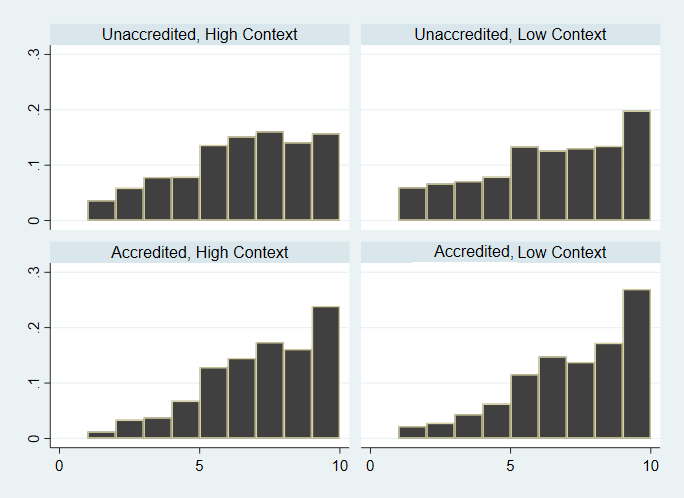
\includegraphics[width=1\textwidth]{./figures-and-tables/context-graph-massaged.png}};
    \end{tikzpicture}
    \label{fig:var_results}
\end{figure}

% This effect does not enter in to any regression
Finally, Figure \ref{fig:var_results} visualizes the prestige response distribution
for actual schools.
Responses are grouped according to whether the respondent randomly received information
from review site aggregators.
For all schools, responses at the positive and negative extrema are both reduced
when individuals are exposed to informational messages.
On average, alternative education prestige rose and accredited education prestige declined
when a respondent received review aggregator site information.

\section{Conclusions}

The results of this paper provide evidence that credential prestige explains a larger share
of hirability variance compared to accreditation.
At the same time, accreditation independently explains a substantial share of hirability.
The independent importance of accreditation indicates that arbitrary improvements to alternative credential
quality and social acceptability will not displace the higher education system.
A change in legal norms appears to be required in order to create an even competitive environment between traditional and alternative providers.

In 2012, The Heritage Foundation called for two policy changes that are worth considering.
First, the Foundation proposed that the government should directly accredit courses rather than organizations\cite{burke2012accreditation}.
Second, they also called for a decoupling of accreditation and federal funding.
An additional option would be to replace legal requirements for formal education could be replaced with skill assessments.
Without a legal requirement for formal education, then, formal accreditation could be removed.

There are several reasons to be pessimistic about the feasibility of these policy changes.
Reductions in public expenditure are particularly unpopular among the voting populace.
Education is compulsory in the United States,
over ninety percent of K-12 students in the United States attended a public school in 2016\cite{us2019digest},
and there is a systematized pipeline from public school to the traditional university system.
Education represents an example of entangled political economy\cite{wagner2014entangled}.
Robust political economy points out additional reasons to doubt rapid innovation in this space\cite{boettke2004liberalism}.

An interesting alternative to formal legislative change is the emerging model of public-private partnership in education.
In 2013, Georgia Tech formally partnered with Udacity to produce an accredited online graduate degree in Computer Science\cite{empson_2013}.
Udacity was able to facilitate a high quality experience online and at scale with an affordable rate.
Georgia Tech offered branding, legitimacy, and accreditation which allowed Udacity to charge a higher price.
In other cases, the hybridization of traditional and alternative education is informal.
Prior learning assessments and portfolio review are two of many processes by which a university can award credit to a student
without formal requirements connected to the source of student learning\cite{conrad2008building}.
This is one route by which course-level accreditation can effectively take place without formal legislative support.

% 1. remove accreditation
% 2. lower the bar for accreditation
% 3. remove professional requirements that include requirement for accreditation
% 4. remove legally enshrined preferential treatment of accredited credentials (esp government pay scales and in government contracts)
% 5. how to fill the gap? define skill-based requirements instead of accreditation (better outcomes for govt and all)
% 6. (institution based vs skill or course based accreditation)
% 1. ...see 8 for a non-policy workaround (but working around is likely more costly than direct fix)
% 6. aggregators need to do a better job
% 7. individuals don't need to wait for social movement to reap individual-level benefits
% 8. hybrid approach; universities can (and increasingly already do) partner with external providers for a win-win
% 1. better university placement rates
% 2. better university solutioning of the skill gap
% 3. accreditation given fully or partially (ACE; professional credit) to unaccredited partners (institution based vs skill or course based accreditation)

Finally, this paper evaluated practical alternative credential selection strategies.
One strategy is to leverage credentials from industry leaders.
Google was selected as a Fortune 50 alternative learning provider.
A credential from Google was the only alternative credential to be identified as generally competitive with an accredited degree.
The second strategy is to use credential review aggregator sites to identify high prestige credentials.
This paper used Course Report as an aggregator to search for alternative credentials.
App Academy and General Assembly were identified by applying search criteria that includes a rating of 4.25 or better on a 5-point scale and a minimum of four hundred reviews.
The combination of results with information on typical job search length from Zety indicated
that these credentials provide meaningful job search benefits,
albeit with significantly less efficacy than an accredited degree or a credential from Google.


\bibliography{./BibFile}

\end{document}
